% ============================================================
% 测评卷小样 v4 · LaTeX 轨（人教B版选必1 §1.1.1 空间向量及其运算）
% 承 v3 题源（10 题：简单6/中档4，题目文字与公式零增删），v4 版式改版：
%   A4 横放 3 栏（栏宽≈84mm、栏距 8mm、无栏线）；卷头瘦身 ≤30mm 占首栏、卷名 16pt；
%   撤页眉；页脚＝单行 #DDDDDD 灰块页码、底缘离页底 ≈11mm；
%   分区标题同号连排（撤 12pt 独立行）；题间距 3pt；选项按长度 4/2/1 项每行（分号字符全保留）；
%   题侧标签＝难度＋（知识点N）＋★（6.5pt #777777，随题号内联＝防折行）；
%   解答题分值移题号后（10．（25分），全品位）；Q6 竖图 TikZ 矢量重绘（图内字号 7.5pt≈正文 71%）；
%   不留作答留白（作答另纸）；\linespread{1} 行距通解＋\raggedcolumns 末页参差；
%   灰档收敛 黑＋777777＋DDDDDD（单页 ≤2 灰档、底线黑、撤栏线）；
%   题号悬挂 7mm 窄列恒空（断言题号列.py 核验）；答案与解析另起页、3 栏密集排。
% 编译：xelatex main.tex（两遍）；渲染：render.py（先清 png/）；断言：断言题号列.py＋断言版式.py
% ============================================================
\documentclass[fontset=none]{ctexart}

% ---------- 字体（同 v3） ----------
\setmainfont{Times New Roman}
\setCJKmainfont[BoldFont=SimHei]{SimSun}   % 宋体正文，加粗映射黑体（无伪粗告警）
\setCJKfamilyfont{hei}{SimHei}
\newcommand{\heiti}{\CJKfamily{hei}}
% 带圈序号/几何符号/★路由给中文字体（Times 无这些字形；★在 2600-26FF 杂项符号区）
\xeCJKDeclareCharClass{CJK}{"2460->"24FF, "2200->"22FF, "25A0->"25FF, "2600->"26FF}
\xeCJKsetup{CheckSingle=true}               % 检测并消除汉字单字孤行

% ---------- 宏包 ----------
\usepackage[a4paper,landscape,top=15mm,bottom=17.33mm,left=15mm,right=15mm,headheight=12pt,headsep=2mm,footskip=3mm]{geometry}
\usepackage{amsmath,amssymb}
\usepackage{graphicx}
\usepackage{xcolor}
\usepackage{multirow,array,calc}
\usepackage{multicol}
\usepackage{needspace}
\usepackage{fancyhdr}
\usepackage{indentfirst}
\usepackage{tikz}

% ---------- 颜色（纯灰阶收敛：黑＋777777＋DDDDDD；撤 v3 的 BFBFBF 栏线与 808080 页眉页脚灰） ----------
\definecolor{pnumbg}{HTML}{DDDDDD}     % 页码灰块（唯一浅灰装饰件）
\definecolor{kygray}{HTML}{777777}     % 题侧标签灰字（难度＋（知识点N）＋★）

% ---------- 版面（v4：横放 3 栏） ----------
% 行距通解（总诊断 #1）：撤 ctex linespread 叠乘，一处归一
\linespread{1}
\renewcommand{\normalsize}{\fontsize{10.5pt}{18pt}\selectfont}
\normalsize
\setlength{\columnsep}{8mm}                 % 栏距 8mm（栏宽 (297-30-16)/3≈83.67mm）
\setlength{\columnseprule}{0pt}             % 撤栏线（测评卷件型）
\setlength{\multicolsep}{0pt}               % 卷头在首栏顶，撤环境前后附加空距
\setlength{\parindent}{2em}
% 孤行寡行治理 + 断行韧性（同 v3）
\clubpenalty=10000
\widowpenalty=10000
\displaywidowpenalty=10000
\tolerance=9999
\binoppenalty=100
\relpenalty=100
\raggedbottom

% ---------- 表格默认（全框细线＋紧凑内边距；本卷无表格，随公共规格保留） ----------
\setlength{\arrayrulewidth}{0.4pt}
\setlength{\tabcolsep}{3pt}
\renewcommand{\arraystretch}{1.3}

% ---------- 页眉页脚（v4：撤页眉；页脚＝单行灰块页码，底缘离页底≈11mm） ----------
% 页脚：单行 #DDDDDD 灰块页码，底缘离页底实测 11.0mm（bottom=17.33mm＋strut[-1.45mm]{5mm}，
% 页码字形纵向居中；灰块顶 16.0mm＜正文底 17.33mm 不侵入）
\newcommand{\footblock}{{\setlength{\fboxsep}{0pt}\colorbox{pnumbg}{%
  \makebox[31mm][c]{\rule[-1.45mm]{0pt}{5mm}\fontsize{10.5pt}{12pt}\selectfont\bfseries\thepage}}}}
\pagestyle{fancy}
\fancyhf{}
\fancyfoot[C]{\footblock}
\renewcommand{\headrulewidth}{0pt}

% ---------- 自定义命令 ----------
% glueguard：multicol 安全的防孤悬软断点（同 v3：无 \break，负伸缩自闭合）
\newcommand{\glueguard}[1]{\vskip 0pt plus #1\baselineskip\penalty-100\vskip 0pt plus -#1\baselineskip}
% 题侧标签（难度＋★＋（知识点N））：6.5pt #777777 灰字，随题号内联＝零强制折行（v4 防折行口径）；
% ★ 为空时不印
\newcommand{\sidemark}[3]{{\fontsize{6.5pt}{8pt}\selectfont\color{kygray}#1#2（知识点#3）}}
% 解答题分值（全品位：题号后「（13分）」式；题号黑体、分值宋体同号）
\newcommand{\fenzhi}[1]{{\mdseries（#1分）}}
% 题号悬挂（同 v3 \timu）：题号顶格，续行内收 7mm；题前 3pt 题间距（v4 降档 6→3pt）
\newcommand{\timu}[5]{\par\glueguard{4}\addvspace{3pt}%
  \noindent\hangindent=7mm\hangafter=1\textbf{#1}\sidemark{#2}{#3}{#4}\,#5\par}
% 题型分区标题：同号 10.5pt 连排（撤 12pt 独立行），黑体前缀＋宋体引导语同段；空距降档 12/3→2/1pt
\newcommand{\quku}[2]{\par\glueguard{6}\addvspace{2pt}%
  \noindent{\heiti #1}#2\par\addvspace{1pt}}
% 【】标签：黑体加粗无底纹（同 v3）
\newcommand{\biaoqian}[1]{{\heiti #1}}
% 挖空留白线（同 v3）：下划线，不用灰底
\newcommand{\kongbai}{\underline{\hspace*{15mm}}}
% 卷头填写栏下划线（v4：栏宽 83.67mm 内一行排下，20mm→12mm）
\newcommand{\juanline}{\underline{\hspace*{12mm}}}
% 答案值下划线（同 v3）
\newcommand{\ansval}[1]{\underline{#1}}
% 答案页条目：题号＋下划线答案值＋解析一段连排；悬挂 7mm；前置 glueguard{3} 防条目头孤行
\newcommand{\daan}[3]{\par\glueguard{3}\addvspace{5pt}%
  \noindent\hangindent=7mm\hangafter=1\textbf{#1}\ansval{#2}\quad #3\par}
% 选项段（拍板21：按长度 4/2/1 项每行，分号字符全保留；与题干续行对齐＝全品位悬挂 7mm；
% \hangafter=0 首行即内收；1 项/行在实参内以 \newline 断行）
\newcommand{\opts}[1]{\par\penalty10000\noindent\hangindent=7mm\hangafter=0#1\par\penalty10000}
% 题图独立成块：30mm 栏内居中，从题号右缘 7mm 起排，段前后 \penalty10000 绑定题块；
% 显式清零悬挂残留（模板坑 #6）
\newcommand{\figblk}[1]{\penalty10000\noindent\hangindent=0pt\hangafter=1\hspace*{7mm}%
  \makebox[\dimexpr\linewidth-7mm\relax][c]{\includegraphics[width=30mm]{#1}}\par\penalty10000}
% TikZ 矢量题图块（Q6 竖图重绘）：落位同 \figblk
\newcommand{\tikblk}[1]{\penalty10000\noindent\hangindent=0pt\hangafter=1\hspace*{7mm}%
  \makebox[\dimexpr\linewidth-7mm\relax][c]{#1}\par\penalty10000}

\begin{document}

\begin{multicols}{3}
\raggedcolumns
% multicol 进入时会把 \emergencystretch 重置为默认 8pt（v2 实测），重设 8em 消巨型公式 overfull
\emergencystretch=8em

% ================= 卷头（v4：瘦身 ≤30mm、占首栏） =================
{\centering
{\fontsize{10.5pt}{13.3pt}\selectfont 班级：\juanline\quad 姓名：\juanline\quad 考号：\juanline\par}
\vspace{1pt}
{\fontsize{16pt}{18pt}\selectfont\heiti 1.1.1\ 空间向量及其运算\par
\vspace{1pt}·\ 节检测卷\par}
\vspace{1pt}
{\fontsize{10.5pt}{13.3pt}\selectfont （时间：45分钟\quad 满分：75分）\par}
\vspace{1pt}
{\fontsize{10.5pt}{13.3pt}\selectfont 考生注意：请在答题纸上作答，答在本卷上无效。\par}
}
\vspace{2pt}

% ================= 正文 3 栏 =================
\quku{一、单选题（每小题5分，共20分）}{本题共4小题。在每小题给出的四个选项中，只有一项是符合题目要求的。}

\timu{1．}{简单}{★}{1}{下列说法正确的是（~~~~）}

\opts{A．若\(\left| \overrightarrow{a} \right| = \allowbreak\left| \overrightarrow{b} \right|\)，则\(\overrightarrow{a} = \overrightarrow{b}\)或\(\overrightarrow{a} = - \overrightarrow{b}\)；\newline B．若\(\overrightarrow{a},\overrightarrow{b}\)为相反向量，则\(\overrightarrow{a} + \overrightarrow{b} = \overrightarrow{0}\)；\newline C．零向量是没有方向的向量；\newline D．若\(\overrightarrow{a},\overrightarrow{b}\)是两个单位向量，则\(\overrightarrow{a} = \overrightarrow{b}\)}

\timu{2．}{简单}{}{3}{有下列说法:}

\opts{①若\(\overrightarrow{p} = x\overrightarrow{a} + y\overrightarrow{b}\)，则\(\overrightarrow{p}\)与\(\overrightarrow{a}\)，\(\overrightarrow{b}\)共面；②若\(\overrightarrow{p}\)与\(\overrightarrow{a}\)，\(\overrightarrow{b}\)共面，则\(\overrightarrow{p}\)=\emph{x}\(\overrightarrow{a}\)+\emph{y}\(\overrightarrow{b}\)；③若\(\overrightarrow{MP}\)=\emph{x}\(\overrightarrow{MA}\)+\emph{y}\(\overrightarrow{MB}\)，则\emph{P}，\emph{M}，\emph{A}，\emph{B}共面；④若\emph{P}，\emph{M}，\emph{A}，\emph{B}共面，则\(\overrightarrow{MP}\)=\emph{x}\(\overrightarrow{MA}\)+\emph{y}\(\overrightarrow{MB}\).其中正确的是（~~~~）}

\opts{A．①②③④；B．①③④；\newline C．①③；D．②④}

\timu{3．}{中档}{}{3}{如图，在大小为45°的二面角A\-EF\-D中，四边形ABFE，CDEF都是边长为1的正方形，则B，D两点间的距离是()}

\figblk{media/image4.png}

\opts{A．\(\sqrt{3}\)；B．\(\sqrt{2}\)；C．1；D．\(\sqrt{3 - \sqrt{2}}\)}

\timu{4．}{中档}{}{3}{已知矩形\(ABCD\)中，\(AB = 1\)，\(BC = \sqrt{3}\)，将矩形\(ABCD\)沿对角线\(AC\)折起，使平面\(ABC\)与平面\(ACD\)垂直，则\(|\overrightarrow{BD}| =\)（~~~~）．}

\opts{A．\(\frac{\sqrt{10}}{2}\)；B．\(\frac{\sqrt{6}}{2}\)；C．\(\frac{\sqrt{5}}{2}\)；D．2}

\figblk{media/image5.png}

\quku{二、多选题（每小题6分，共6分）}{本题共1小题。在每小题给出的选项中，有多项符合题目要求。全部选对的得6分，部分选对的得部分分，有选错的得0分。}

\timu{5．}{简单}{★}{3}{设\(\overrightarrow{a}\)，\(\overrightarrow{b}\)为空间中的任意两个非零向量，下列各式中正确的有（~~~~）}

\opts{A．\({\overrightarrow{a}}^{2} = \allowbreak\left| \overrightarrow{a} \right|^{2}\)；\newline B．\(\frac{\overrightarrow{a} \cdot \overrightarrow{b}}{\overrightarrow{a} \cdot \overrightarrow{a}} = \frac{\overrightarrow{b}}{\overrightarrow{a}}\)；\newline C．\(\left( \overrightarrow{a} \cdot \overrightarrow{b} \right)^{2} = {\overrightarrow{a}}^{2} \cdot {\overrightarrow{b}}^{2}\)；\newline D．\(\left( \overrightarrow{a} - \overrightarrow{b} \right)^{2} = {\overrightarrow{a}}^{2} - 2\overrightarrow{a} \cdot \overrightarrow{b} + {\overrightarrow{b}}^{2}\)}

\quku{三、填空题（每小题6分，共24分）}{本题共4小题。}

\timu{6．}{简单}{}{2}{在直三棱柱\(ABC - A_{1}B_{1}C_{1}\)中，若\(\overrightarrow{CA} = \overrightarrow{a},\overrightarrow{CB} = \overrightarrow{b},\overrightarrow{CC_{1}} = \overrightarrow{c},\)，则\(\overrightarrow{A_{1}B}\)=\kongbai.(用\(\overrightarrow{a},\overrightarrow{b},\overrightarrow{c}\)表示)}

\tikblk{%
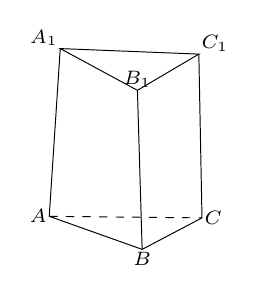
\begin{tikzpicture}[x=1mm,y=1mm,line width=0.35pt,
  every node/.style={font=\fontsize{7.5pt}{8.5pt}\selectfont,inner sep=0.8pt}]
  \coordinate (A1) at (2.2,25.5);
  \coordinate (C1) at (19.8,24.8);
  \coordinate (B1) at (12.0,20.2);
  \coordinate (A)  at (0.8,4.2);
  \coordinate (C)  at (20.2,4.0);
  \coordinate (B)  at (12.6,0);
  \draw (A1) -- (C1) -- (B1) -- cycle;
  \draw (A) -- (B) -- (C);
  \draw[dashed] (A) -- (C);
  \draw (A) -- (A1);
  \draw (B) -- (B1);
  \draw (C) -- (C1);
  \node[above left]  at (A1) {$A_1$};
  \node[above right] at (C1) {$C_1$};
  \node[above]       at (B1) {$B_1$};
  \node[left]        at (A)  {$A$};
  \node[right]       at (C)  {$C$};
  \node[below]       at (B)  {$B$};
\end{tikzpicture}}

\timu{7．}{简单}{}{2}{已知正方体\emph{ABCD}－\emph{A\textsubscript{1}B\textsubscript{1}C\textsubscript{1}D\textsubscript{1}}中，\(\overrightarrow{A_{1}E}\)＝\(\frac{1}{4}\) \(\overrightarrow{A_{1}C_{1}}\)，若\(\overrightarrow{AE} =\)\emph{x}\(\overrightarrow{AA_{1}}\)＋\emph{y}(\(\overrightarrow{AB}\)＋\(\overrightarrow{AD}\))，则\emph{x}＝\kongbai，\emph{y}＝\kongbai.}

\figblk{media/image2.png}

\timu{8．}{中档}{★}{3}{已知向量\(\overrightarrow{a},\overrightarrow{b}\)，且\(\left| \overrightarrow{a} \right| = 2\)，\(\left| \overrightarrow{b} \right| = 1\)，\(\left\langle \overrightarrow{a},\overrightarrow{b} \right\rangle = 60^{\circ}\)，则使向量\(\overrightarrow{a} + \lambda\overrightarrow{b}\)与\(\lambda\overrightarrow{a} - 2\overrightarrow{b}\)的夹角为钝角的实数\(\lambda\)的取值范围是\kongbai．}

\timu{9．}{简单}{}{3}{已知\(\left| \overrightarrow{a} \right| = 3\sqrt{2},\left| \overrightarrow{b} \right| = 4,\)\(\overrightarrow{m} = \overrightarrow{a} + \overrightarrow{b},\overrightarrow{n} = \overrightarrow{a} + \lambda\overrightarrow{b},\left\langle \overrightarrow{a},\overrightarrow{b} \right\rangle = 135{^\circ},\overrightarrow{m}\bot\overrightarrow{n}\) ，则λ＝\kongbai．}

\quku{四、解答题}{本题共1小题。解答应写出文字说明、证明过程或演算步骤。}

\timu{10．\fenzhi{25}}{中档}{}{3}{如图，在正方体\(ABCD - A_{1}B_{1}C_{1}D_{1}\)中，求向量\(\overrightarrow{BC_{1}}\)与\(\overrightarrow{AC}\)的夹角的大小．}

\figblk{media/image3.png}

\end{multicols}

% ================= 答案与解析（另起页，3 栏密集排） =================
\clearpage
{\centering
{\fontsize{15pt}{22pt}\selectfont\heiti 参考答案与解析\par}
\vspace{3pt}\noindent\rule{\textwidth}{0.4pt}\par}
\vspace{4pt}

\begin{multicols}{3}
\raggedcolumns
\emergencystretch=8em

\daan{1．}{B}{\biaoqian{【分析】}根据零向量、单位向量、向量的模、相等向量、相反向量等概念逐一分析即可得出答案.\biaoqian{【详解】}解：若\(\left| \overrightarrow{a} \right| = \allowbreak\left| \overrightarrow{b} \right|\)，则它们的方向相同时是相等向量，方向相反时是相反向量，还有可能方向既不相同，也不相反，A错；若\(\overrightarrow{a},\overrightarrow{b}\)为相反向量，则它们的和为零向量，B对；零向量的方向是任意的，C错；两个单位向量只是模都为1，方向不一定相同，D错.故选：B.}

\daan{2．}{C}{\biaoqian{【分析】}利用空间向量共面定理逐一判断即可.\biaoqian{【详解】}若\(\overrightarrow{a}\)，\(\overrightarrow{b}\)共线，由\(\overrightarrow{p}\)=\emph{x}\(\overrightarrow{a}\)+\emph{y}\(\overrightarrow{b}\)知\(\overrightarrow{p}\)一定与\(\overrightarrow{a}\)，\(\overrightarrow{b}\)共面，若\(\overrightarrow{a}\)，\(\overrightarrow{b}\)不共线，则满足共面定理，\(\overrightarrow{p}\)与\(\overrightarrow{a}\)，\(\overrightarrow{b}\)共面，①对；同理③对；若\(\overrightarrow{p}\)与\(\overrightarrow{a}\)，\(\overrightarrow{b}\)共面，且\(\overrightarrow{a}\)，\(\overrightarrow{b}\)共线，则不一定有\(\overrightarrow{p}\)=\emph{x}\(\overrightarrow{a}\)+\emph{y}\(\overrightarrow{b}\)，故②不对；同理④不对，故选：C.}

\daan{3．}{D}{\biaoqian{【分析】}由\(\overrightarrow{DB} = \overrightarrow{ED} + \overrightarrow{FE} + \overrightarrow{BF}\)，利用数量积运算性质展开即可得到答案\biaoqian{【详解】}\(\because\overrightarrow{BD} = \overrightarrow{ED} + \overrightarrow{FE} + \overrightarrow{BF}\),\(\therefore\left| \overrightarrow{BD} \right|^{2} = \allowbreak\left| \overrightarrow{BF} \right|^{2} + \left| \overrightarrow{FE} \right|^{2} + \left| \overrightarrow{ED} \right|^{2} + 2\overrightarrow{BF} \bullet \overrightarrow{FE} + 2\overrightarrow{FE} \bullet \overrightarrow{ED} + 2\overrightarrow{BF} \bullet \overrightarrow{ED} = 1 + 1 + 1 - \sqrt{2}\)故\(\left| \overrightarrow{BD} \right| = \sqrt{3 - \sqrt{2}}\)故选\(D\)\biaoqian{【点睛】}本题是要求空间两点之间的距离，运用空间向量将其表示，然后计算得到结果，较为基础．}

\daan{4．}{A}{\biaoqian{【分析】}过点\(B\)，\(D\)分别向\(AC\)作垂线，垂足分别为\(M\)，\(N\)，由\(\overrightarrow{BD} = \overrightarrow{BM} + \overrightarrow{MN} + \overrightarrow{ND}\)，平方后结合长度和垂直关系可得解.\biaoqian{【详解】} ~~过点\(B\)，\(D\)分别向\(AC\)作垂线，垂足分别为\(M\)，\(N\)，则可得\(AM = \frac{1}{2}\)，\(BM = \frac{\sqrt{3}}{2}\)，\(CN = \frac{1}{2}\)，\(DN = \frac{\sqrt{3}}{2}\)，\(MN = 1\)．由于\(\overrightarrow{BD} = \overrightarrow{BM} + \overrightarrow{MN} + \overrightarrow{ND}\)，所以\(|\overrightarrow{BD}|^{2} = {(\overrightarrow{BM} + \overrightarrow{MN} + \overrightarrow{ND})}^{2}\)\(= |\overrightarrow{BM}|^{2} + |\overrightarrow{MN}|^{2} + |\overrightarrow{ND}|^{2} + 2(\overrightarrow{BM} \cdot \overrightarrow{MN} + \overrightarrow{MN} \cdot \overrightarrow{ND} + \overrightarrow{BM} \cdot \overrightarrow{ND})\)\(= \left( \frac{\sqrt{3}}{2} \right)^{2} + 1^{2} + \left( \frac{\sqrt{3}}{2} \right)^{2} + 2 \times (0 + 0 + 0) = \frac{5}{2}\)，所以\(|\overrightarrow{BD}| = \frac{\sqrt{10}}{2}\)．故选:\emph{A}．\biaoqian{【点睛】}本题主要考查了空间向量数量积的应用，属于基础题.}

\daan{5．}{AD}{\biaoqian{【分析】}根据空间向量数量积的定义与运算律一一判断即可；\biaoqian{【详解】}解：对于A：\({\overrightarrow{a}}^{2} = \overrightarrow{a} \cdot \overrightarrow{a} = \allowbreak\left| \overrightarrow{a} \right| \cdot \allowbreak\left| \overrightarrow{a} \right|\cos 0 = \allowbreak\left| \overrightarrow{a} \right|^{2}\)，故A正确；对于B：因为向量不能做除法，即\(\frac{\overrightarrow{b}}{\overrightarrow{a}}\)无意义，故B错误；对于C：\(\left( \overrightarrow{a} \cdot \overrightarrow{b} \right)^{2} = \allowbreak\left( \left| \overrightarrow{a} \right| \cdot \allowbreak\left| \overrightarrow{b} \right|\cos\left\langle \overrightarrow{a},\overrightarrow{b} \right\rangle \right)^{2} = \allowbreak\left| \overrightarrow{a} \right|^{2} \cdot \allowbreak\left| \overrightarrow{b} \right|^{2}\cos^{2}\left\langle \overrightarrow{a},\overrightarrow{b} \right\rangle\)，故C错误；对于D：\(\left( \overrightarrow{a} - \overrightarrow{b} \right)^{2} = \allowbreak\left( \overrightarrow{a} - \overrightarrow{b} \right) \cdot \allowbreak\left( \overrightarrow{a} - \overrightarrow{b} \right) = {\overrightarrow{a}}^{2} - 2\overrightarrow{a} \cdot \overrightarrow{b} + {\overrightarrow{b}}^{2}\)，故D正确；故选：AD}

\daan{6．}{\(\overrightarrow{b} - \overrightarrow{a} - \overrightarrow{c}\)}{\biaoqian{【分析】}连接\(CA_{1},\)根据直三棱柱的结构特征及空间向量减法的几何意义可得\(\overrightarrow{A_{1}B} = \overrightarrow{CB} - \overrightarrow{CA} - \overrightarrow{CC_{1}}\)，结合已知即可求表达式.\biaoqian{【详解】}连接\(CA_{1},\)则\(\overrightarrow{A_{1}B} = \overrightarrow{CB} - \overrightarrow{CA_{1}} = \overrightarrow{CB} - \overrightarrow{CA} - \overrightarrow{CC_{1}} =\)
\(\overrightarrow{b} - \overrightarrow{a} - \overrightarrow{c}\).故答案为：\(\overrightarrow{b} - \overrightarrow{a} - \overrightarrow{c}\)}

\daan{7．}{\(1\)；\(\frac{1}{4}\)}{\biaoqian{【分析】}结合空间向量的线性运算列方程，由此求得\(x,y\)的值.\biaoqian{【详解】}\(\overrightarrow{AE} = \overrightarrow{AA_{1}} + \overrightarrow{A_{1}E} = \overrightarrow{AA_{1}} + \frac{1}{4}\overrightarrow{A_{1}C_{1}} = \overrightarrow{AA_{1}} + \frac{1}{4}\left( \overrightarrow{AB} + \overrightarrow{AD} \right)\)，所以\(x = 1,y = \frac{1}{4}\).故答案为：\(1\)；\(\frac{1}{4}\)}

\daan{8．}{\(\left( - 1 - \sqrt{3}, - 1 + \sqrt{3} \right)\)}{\biaoqian{【分析】}根据\(\left( \overrightarrow{a} + \lambda\overrightarrow{b} \right) \cdot \allowbreak\left( \lambda\overrightarrow{a} - 2\overrightarrow{b} \right) < 0\)，得出方程求得\(- 1 - \sqrt{3} < \lambda < - 1 + \sqrt{3}\)，若向量\(\overrightarrow{a} + \lambda\overrightarrow{b}\)与\(\lambda\overrightarrow{a} - 2\overrightarrow{b}\)反向共线时，则存在实数\(k < 0\)使得\(\overrightarrow{a} + \lambda\overrightarrow{b} = k(\lambda\overrightarrow{a} - 2\overrightarrow{b})\)成立，得到方程组\(\left\{ \begin{array}{r}
k\lambda = 1 \\
\lambda = - 2k
\end{array} \right.\ \)无解，即可得到答案.\biaoqian{【详解】}由向量\(\overrightarrow{a},\overrightarrow{b}\)，且\(\left| \overrightarrow{a} \right| = 2\)，\(\left| \overrightarrow{b} \right| = 1\)，\(\left\langle \overrightarrow{a},\overrightarrow{b} \right\rangle = 60^{\circ}\)，可得\(\overrightarrow{a} \cdot \overrightarrow{b} = 2 \times 1 \times \cos 60^{\circ} = 1\)，因为向量\(\overrightarrow{a} + \lambda\overrightarrow{b}\)与\(\lambda\overrightarrow{a} - 2\overrightarrow{b}\)的夹角为钝角，可得\(\cos\left\langle \overrightarrow{a} + \lambda\overrightarrow{b},\lambda\overrightarrow{a} - 2\overrightarrow{b} \right\rangle < 0\)且\(\cos\left\langle \overrightarrow{a} + \lambda\overrightarrow{b},\lambda\overrightarrow{a} - 2\overrightarrow{b} \right\rangle \neq - 1\)，由\(\left( \overrightarrow{a} + \lambda\overrightarrow{b} \right) \cdot \allowbreak\left( \lambda\overrightarrow{a} - 2\overrightarrow{b} \right) < 0\)，即\(\lambda{\overrightarrow{a}}^{2}\text{+(}\lambda^{2} - 2)\overrightarrow{a} \cdot \overrightarrow{b} - 2\lambda{\overrightarrow{b}}^{2} < 0\)，所以\(\lambda^{2} + 2\lambda - 2 < 0\)，解得\(- 1 - \sqrt{3} < \lambda < - 1 + \sqrt{3}\)，若向量\(\overrightarrow{a} + \lambda\overrightarrow{b}\)与\(\lambda\overrightarrow{a} - 2\overrightarrow{b}\)反向共线时，存在实数\(k < 0\)，使得\(\overrightarrow{a} + \lambda\overrightarrow{b} = k(\lambda\overrightarrow{a} - 2\overrightarrow{b})\)成立，可得\(\left\{ \begin{array}{r}
k\lambda = 1 \\
\lambda = - 2k
\end{array} \right.\ \)，此时方程组无解，所以不存在实数\(k\)使得向量\(\overrightarrow{a} + \lambda\overrightarrow{b}\)与\(\lambda\overrightarrow{a} - 2\overrightarrow{b}\)反向共线，所以实数\(\lambda\)的取值范围是\(\left( - 1 - \sqrt{3}, - 1 + \sqrt{3} \right)\).}

\daan{9．}{\(- \frac{3}{2}\)}{\biaoqian{【分析】}根据题意\(\overrightarrow{m}\bot\overrightarrow{n}\)得到\(\left( \overrightarrow{a} + \overrightarrow{b} \right) \cdot \allowbreak\left( \overrightarrow{a} + \lambda\overrightarrow{b} \right) = 0\)，从而可求出\(\lambda\)的值.\biaoqian{【详解】}由\(\overrightarrow{m}\bot\overrightarrow{n}\)，得\(\left( \overrightarrow{a} + \overrightarrow{b} \right) \cdot \allowbreak\left( \overrightarrow{a} + \lambda\overrightarrow{b} \right) = 0\)，即\({\overrightarrow{a}}^{2} + (\lambda + 1) \cdot \overrightarrow{a} \cdot \overrightarrow{b} + \lambda{\overrightarrow{b}}^{2} = 0\)，即
\(\left| \overrightarrow{a} \right|^{2} + (\lambda + 1) \cdot \allowbreak\left| \overrightarrow{a} \right| \cdot \allowbreak\left| \overrightarrow{b} \right| \cdot \cos\left\langle \overrightarrow{a},\overrightarrow{b} \right\rangle + \lambda\left| \overrightarrow{b} \right|^{2} = 0\)，所以\(18 + (\lambda + 1) \times 3\sqrt{2} \times 4 \times \cos 135{^\circ} + 16\lambda = 0\)，即4\emph{λ}＋6＝0，∴\emph{λ}＝\(- \frac{3}{2}\)．故答案为：\(- \frac{3}{2}\).}

\daan{10．}{\(60{^\circ}\)}{\biaoqian{【分析】}方法1：结合图形，平移向量，利用空间向量的夹角定义来求，但要注意向量夹角的范围；方法2：先求\(\overrightarrow{BC_{1}} \cdot \overrightarrow{AC}\)，再利用公式\(\cos\left\langle \overrightarrow{BC_{1}},\overrightarrow{AC} \right\rangle = \frac{\overrightarrow{BC_{1}} \cdot \overrightarrow{AC}}{\left| \overrightarrow{BC_{1}} \right| \cdot \allowbreak\left| \overrightarrow{AC} \right|}\)求\(\cos\left\langle \overrightarrow{BC_{1}},\overrightarrow{AC} \right\rangle\)，最后确定\(\left\langle \overrightarrow{BC_{1}},\overrightarrow{AC} \right\rangle\)即可．\biaoqian{【详解】}解：方法1：因为\(\overrightarrow{AD_{1}} = \overrightarrow{BC_{1}}\)，所以\(\angle CAD_{1}\)的大小就等于\(\left\langle \overrightarrow{BC_{1}},\overrightarrow{AC} \right\rangle\)因为△\(CAD_{1}\)为等边三角形，所以\(\angle CAD_{1} = 60^{{^\circ}}\)，所以\(\overrightarrow{BC_{1}}\)与\(\overrightarrow{AC}\)的夹角的大小为\(60{^\circ}\)．方法2．设正方体的棱长为1，\(\overrightarrow{BC_{1}} \cdot \overrightarrow{AC} = \allowbreak\left( \overrightarrow{BC} + \overrightarrow{CC_{1}} \right) \cdot \allowbreak\left( \overrightarrow{AB} + \overrightarrow{BC} \right) = \allowbreak\left( \overrightarrow{AD} + \overrightarrow{AA_{1}} \right) \cdot \allowbreak\left( \overrightarrow{AB} + \overrightarrow{AD} \right)\)\(= \overrightarrow{AD} \cdot \overrightarrow{AB} + \left| \overrightarrow{AD} \right|^{2} + \overrightarrow{AA_{1}} \cdot \overrightarrow{AB} + \overrightarrow{AA_{1}} \cdot \overrightarrow{AD} = 0 + \left| \overrightarrow{AD} \right|^{2} + 0 + 0 = \allowbreak\left| \overrightarrow{AD} \right|^{2} = 1\)又因为\(\left| \overrightarrow{BC_{1}} \right| = \sqrt{2},\left| \overrightarrow{AC} \right| = \sqrt{2}\)，所以\(\cos\left\langle \overrightarrow{BC_{1}},\overrightarrow{AC} \right\rangle = \frac{\overrightarrow{BC_{1}} \cdot \overrightarrow{AC}}{\left| \overrightarrow{BC_{1}} \right| \cdot \allowbreak\left| \overrightarrow{AC} \right|} = \frac{1}{\sqrt{2} \times \sqrt{2}} = \frac{1}{2}\)，
因为\(\left\langle \overrightarrow{BC_{1}},\overrightarrow{AC} \right\rangle \in \lbrack 0,\pi\rbrack\)，所以\(\overrightarrow{BC_{1}}\)与\(\overrightarrow{AC}\)的夹角的大小为\(60{^\circ}\)．}

\end{multicols}
\end{document}
